\documentclass[]{article}
\usepackage[margin=1in]{geometry}                	
\usepackage{graphicx}			
\usepackage{caption}

\setlength\parindent{0pt} % No indent automatically.
%opening
\title{}
\author{}
\date{}

\begin{document}

\renewcommand{\thefigure}{S\arabic{figure}}
\setcounter{figure}{0}

\begin{figure}[h]
	\centering
	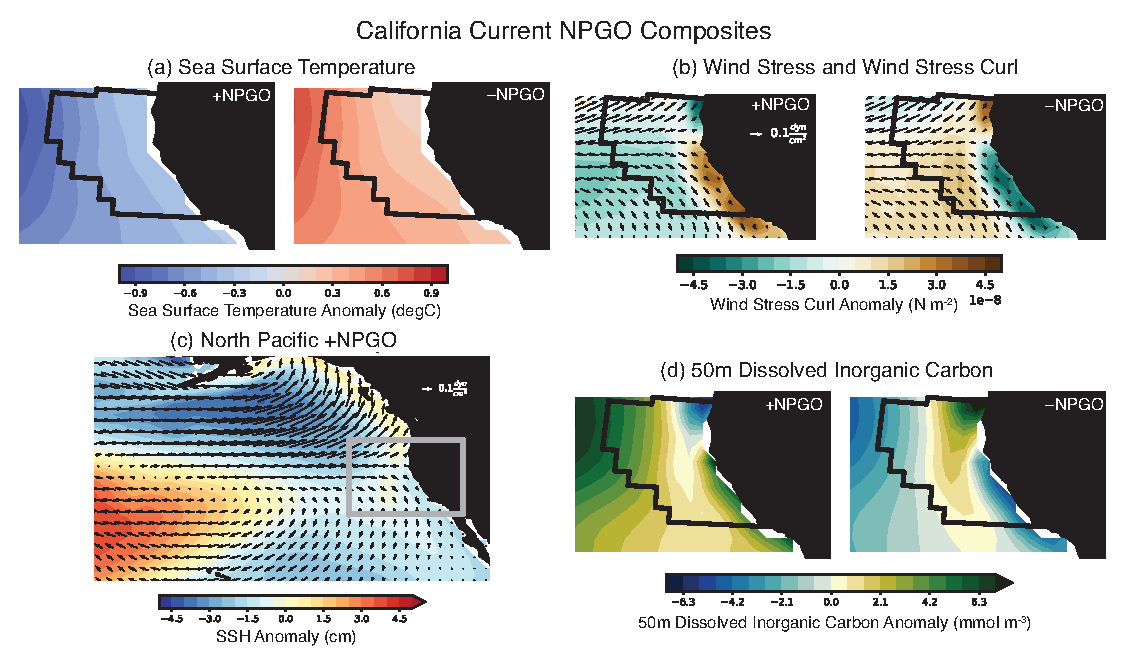
\includegraphics[width=39pc]{figs/S3_CalCS_NPGO_composites.eps}
	\caption{CalCS composites for the positive and negative phase of the NPGO for (a) sea surface temperature, (b) wind stress and wind stress curl, and (d) 50m dissolved inorganic carbon anomalies. The black outline in these plots shows our statistical study region. The positive NPGO forcing pattern for the North Pacific is displayed in (c) for wind stress and sea surface height anomalies. The gray box in (c) delineates the region displayed in (a), (b), and (c). Composites were calculated by averaging every NPGO event that exceeded two standard deviations above or below the index mean for the full ensemble.}
\end{figure}

\newpage
\begin{figure}[h]
	\centering
	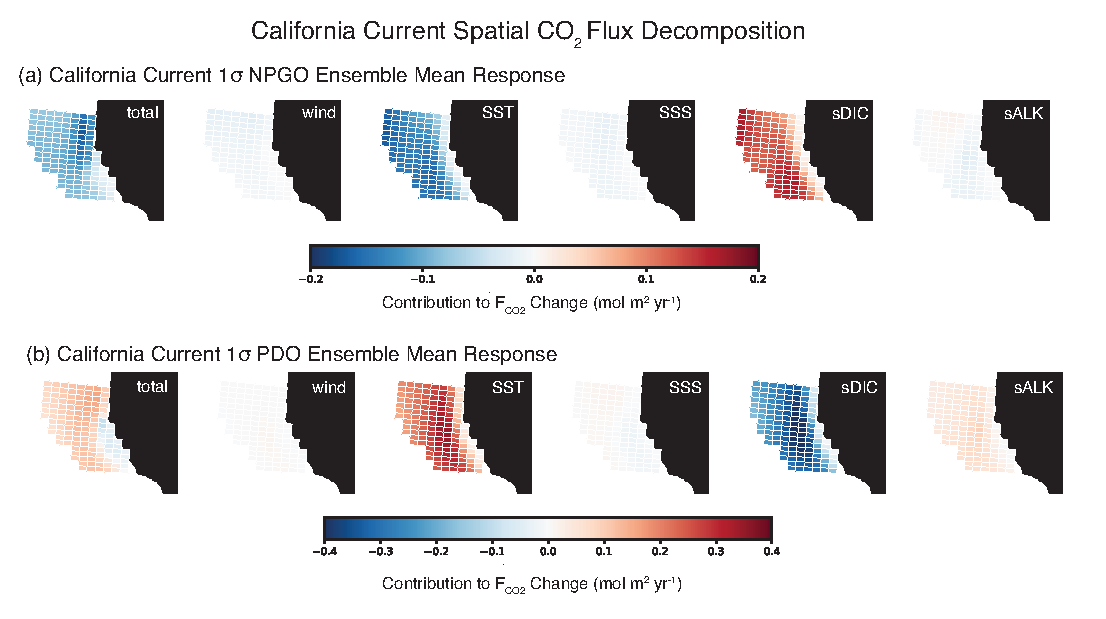
\includegraphics[width=39pc]{figs/S1_overhead_CO2_decomposition.eps}
	\caption{Linear Taylor expansion by grid cell for CO$_{2}$ flux anomalies in the CalCS in response to (a) a 1$\sigma$ NPGO and (b) a 1$\sigma$ PDO.}
\end{figure}

\newpage
\begin{figure}[h]
	\centering
	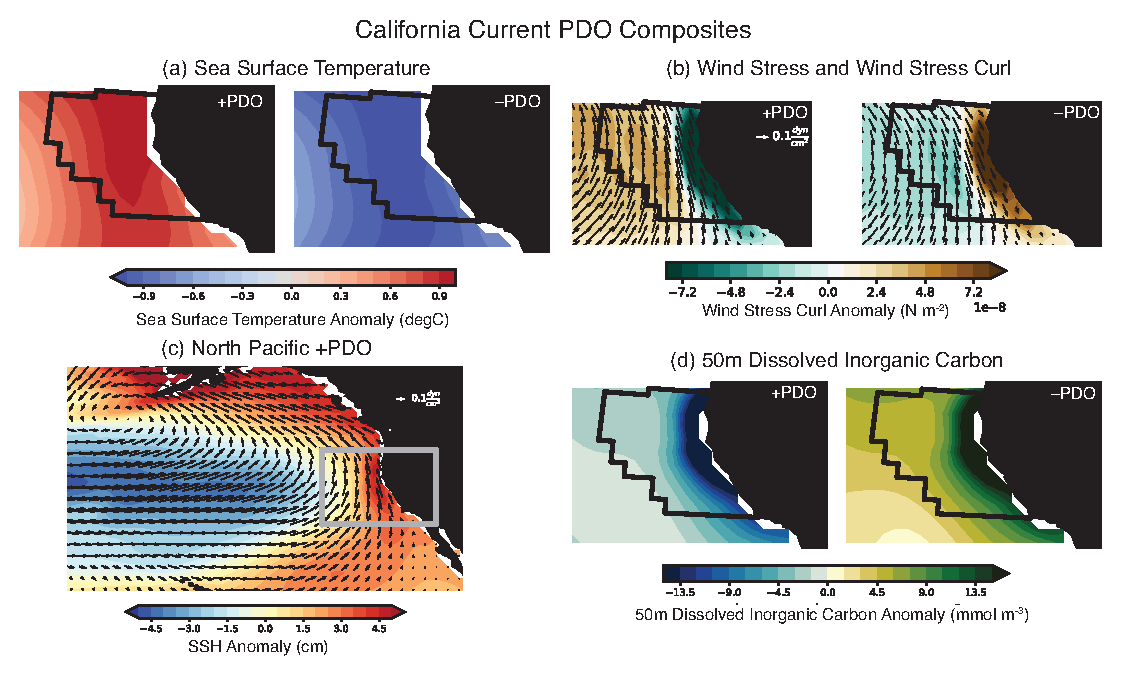
\includegraphics[width=39pc]{figs/S4_CalCS_PDO_composites.eps}
	\caption{As in Figure S1, but for the PDO.}
\end{figure}

\newpage
\begin{figure}[h]
	\centering
	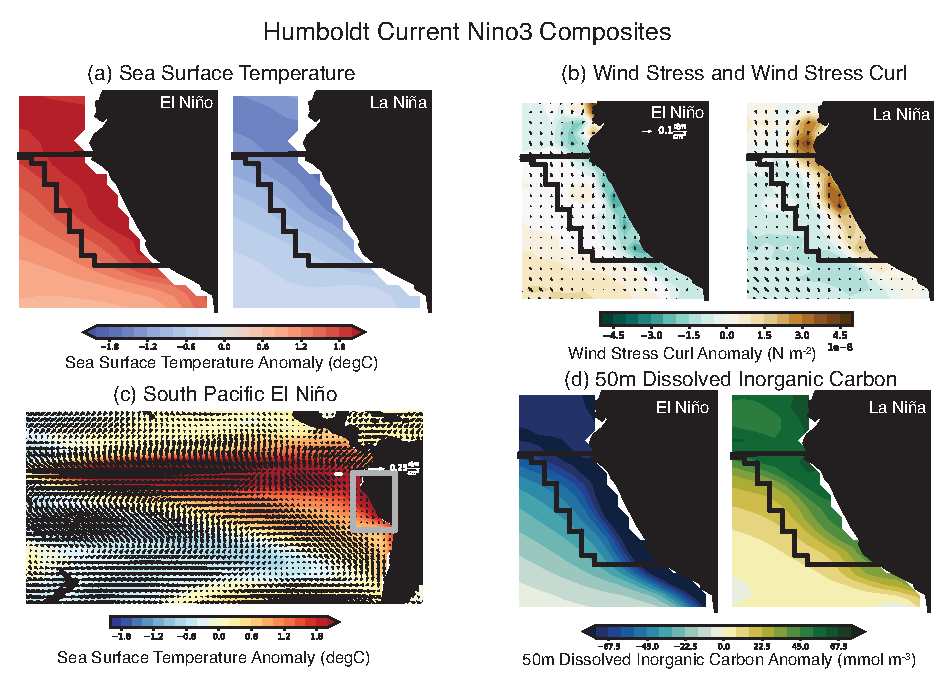
\includegraphics[width=39pc]{figs/S6_HumCS_nino3_composites.eps}
	\caption{As in Figure S1, but for the HumCS response to ENSO.}
\end{figure}

\newpage
\begin{figure}[h]
	\centering
	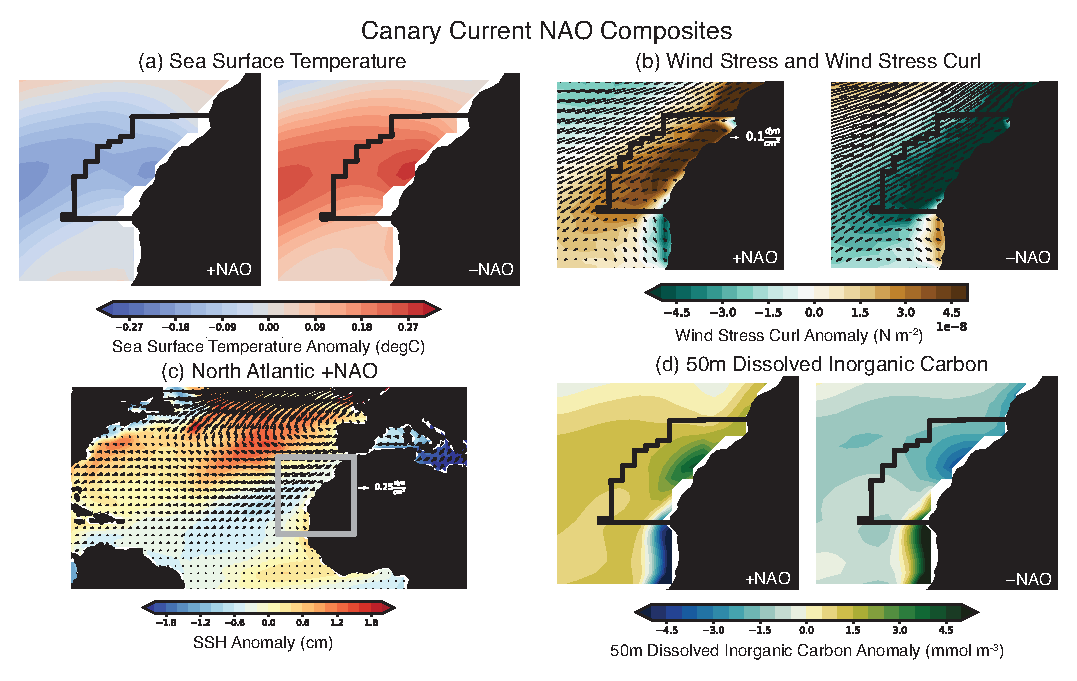
\includegraphics[width=39pc]{figs/S5_CanCS_NAO_composites.eps}
	\caption{As in Figure S1, but for the CanCS response to the NAO.}
\end{figure}


\newpage
\begin{figure}[h]
	\centering
	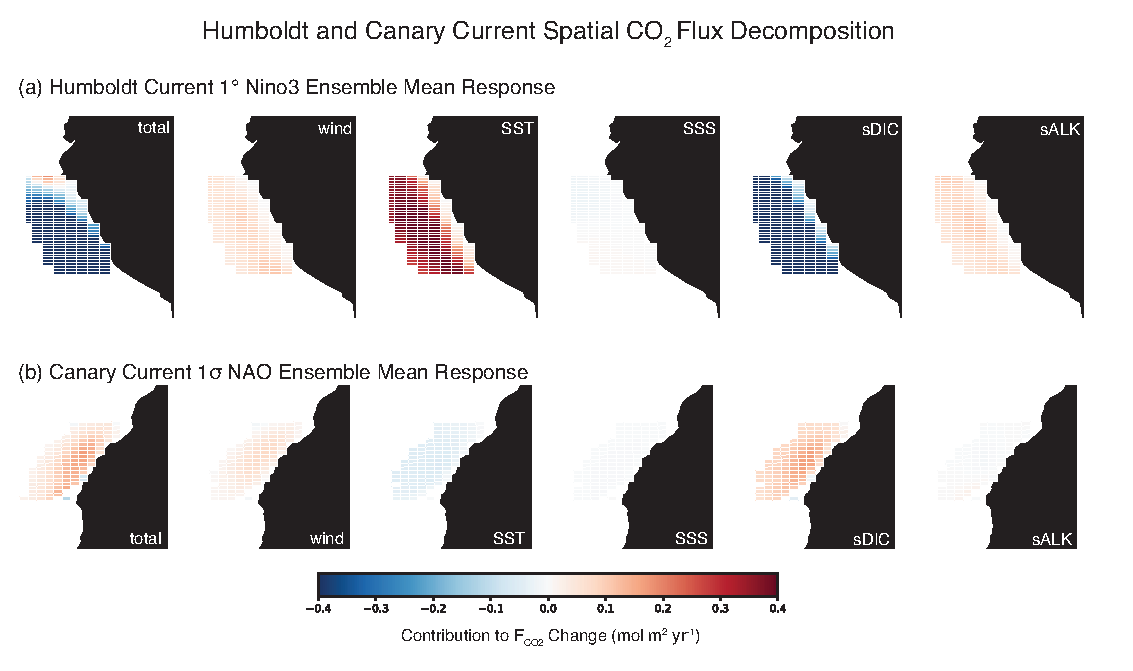
\includegraphics[width=39pc]{figs/S2_CanCS_HumCS_CO2_decomposition.eps}
	\caption{As in Figure S2, but for (a) the HumCS response to ENSO, and (b) the CanCS response to the NAO.}
\end{figure}

\newpage
\begin{figure}[h]
	\centering
	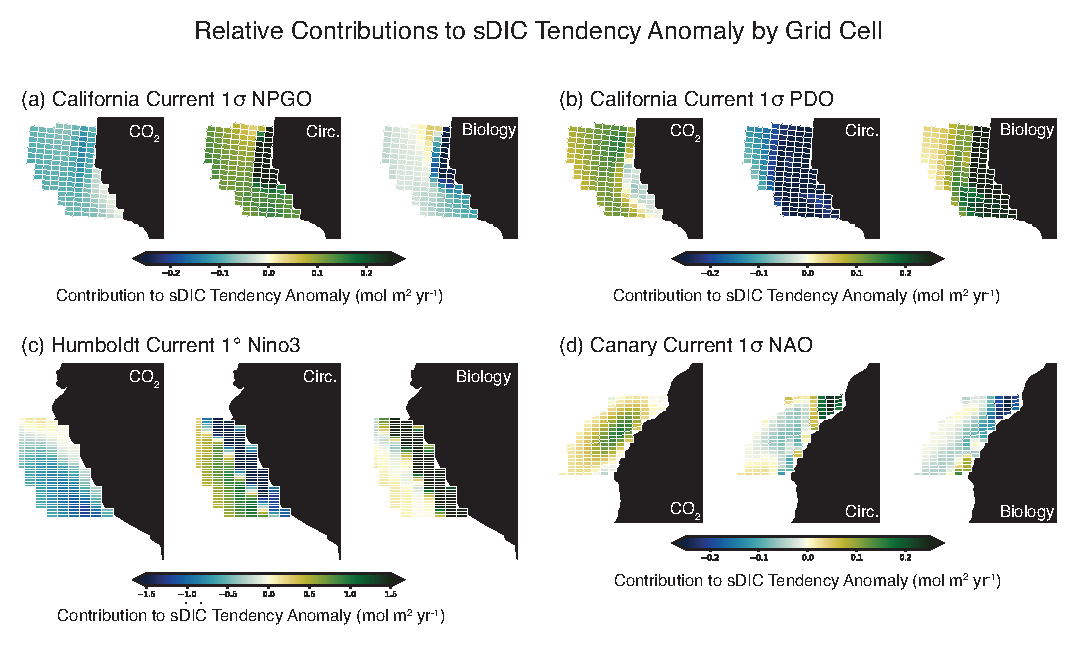
\includegraphics[width=39pc]{figs/S7_sDIC_overhead.eps}
	\caption{Grid cell analysis of the relative contributions to the sDIC tendency anomaly for (a) the CalCS response to the NPGO, (b) the CalCS response to the PDO, (c) the HumCS response to ENSO, and (d) the CanCS response to the NAO. Each subplot contains (from left to right) the relative contribution of CO$_{2}$ flux, circulation, and biology anomalies.}
\end{figure}

\end{document}
